\input{latex-parts/00-preambula}

\begin{document}

\includepdf[page=1, pagecommand={\thispagestyle{plain}}]{pregen}
% \includepdf[page=2, pagecommand={\thispagestyle{plain}}]{pregen}
% \includepdf[page=3, pagecommand={\thispagestyle{plain}}]{pregen}
\setcounter{page}{4}
\ssr{РЕФЕРАТ}

\textbf{Курсовая работа} 47 c., 8 рис., 13 ист., 2 табл., 2 прил.

\textbf{Ключевые слова:} СУБД, БД, Postgresql, minIO, Python

\textbf{Цель работы:}
\textbf{Результаты работы:}

\begin{itemize}
	\item проведён анализ предметной области;
	\item формализованы данные и роли пользователей;
	\item спроектирована и разработана база данных, описаны её сущности и
	      связи;
	\item спроектирован и разработан триггер валидации карты;
	\item спроектирована и разработана хранимая процедура проверки покупки
	      карты;
	\item реализован сайт, использующий базу данных;
	\item проведено исследование зависимости времени формирования
	      персональной колоды от количества карт игрока и структуры данных
	      их хранения.
\end{itemize}

Исследование показало, что производительность операций формирования руки игрока
зависит как от размера колоды, так и от используемой структуры данных. При
больших размерах колод структура \texttt{deque} обеспечивает более высокую
производительность, а наиболее затратной операцией является перемешивание
колоды.
\clearpage


\setlength{\cftsecindent}{0cm}
\def\contentsname{\begin{center} \vspace{-3.4cm}
        Содержание\end{center}}
\tableofcontents

\ssr{ВВЕДЕНИЕ}

Современные многопользовательские онлайн-приложения предъявляют высокие
требования
как к структуре данных, так и к надёжности бизнес-логики и доступности сервиса.
В играх с коллекционированием карт важны производительность операций с
колодами,
правильность валидации данных карт и надёжный контроль прав доступа для разных
ролей
пользователей.

Целью данной работы является разработка базы данных для прототипа игры
<<Эпичные
схватки боевых магов: Крутагидон>>.

Для достижения поставленной цели необходимо решить следующие задачи:

\begin{enumerate}
	\item проанализировать предметную область;
	\item формализовать модель данных и выделить роли пользователей;
	\item спроектировать базу данных, описать её сущности и связи;
	\item выбрать систему управления базами данных;
	\item реализовать базу данных и сайт с игрой;
	\item провести исследование производительности операций с колодами.
\end{enumerate}

\clearpage

\chapter{Аналитическая часть}

В аналитической части проведён анализ предметной области онлайн-версии
настольной игры <<Эпичные схватки боевых магов: Крутагидон>>, в том числе
описание типов карт, механики работы рынка и условий победы. Сформулированы
требования и ограничения к приложению, формализованы данные и роли
пользователей.

\section{Описание предметной области}

Онлайн-версия упомянутой колодостроительной (deck-building) игры представляет
собой многопользовательскую карточную игру, в которой игроки сражаются между
собой, используя карты из общей системы карт. Для реализации используются
механики, описанные в правилах игры, но некоторые объекты
переименованы~\cite{rules}.

Игровой процесс строится на последовательности ходов \textit{игроков} ---
участников игровой сессии, обладающих параметрами состояния (например,
здоровье, очки крутости) и взаимодействующих с игровыми объектами в процессе
игры. Во время своего хода игрок может разыгрывать карты из своей руки,
получать игровой ресурс --- \textit{эхо} --- и использовать его для покупки
новых карт из рынка. Купленные карты добавляются в личную колоду игрока и могут
быть использованы в дальнейшем. В конце каждого хода все карты, с которыми
игрок начинал свой ход, сбрасываются, а на руку набираются новые~\cite{rules}.

Игрок обладает личной колодой карт, которая используется в процессе игры.
Колода формируется из стартовых карт (началок), а затем пополняется новыми
картами, приобретёнными игроком на рынке. Механика работы рынка приведена ниже.
В ходе игры карты могут находиться в различных состояниях (колодах): рука,
добор, стол, сброс, рынок, основная колода и игровой сброс~\cite{rules}.

Типы колод:
\begin{itemize}
	\item рука (hand) --- просматриваемые и разыгрываемые карты, с которыми
	      игрок начинает ход;
	\item колода добора (draw) --- колода игрока, из которой формируется
	      рука и осуществляется добор карт;
	\item стол (table) --- карты, которые игрок разыграл на текущем ходу,
	      доступны к просмотру всем игрокам;
	\item сброс (discard) --- колода для сброшенных карт, формирует колоду
	      добора, когда в ней заканчиваются карты;
	\item рынок (market) --- колода из 5 открытых карт, которые доступны
	      для просмотра всем игроками и покупки игроку в свой ход;
	\item основная игровая колода (deck) --- колода, из которой формируется
	      рынок;
	\item сброс игры (banish) --- карты, которые сбрасываются без возврата
	      в игру.
\end{itemize}

В течение ходов игроки могут получать урон от атак других игроков или атаковать
самостоятельно, пополнять руку новыми картами, лечиться, набирать внутриигровую
валюту покупки карт --- эхо. Атаки уменьшают количество очков здоровья игрока
и, если здоровье игрока становится меньше или равно 0, то игрок на этом ходу
умирает, получает <<памятку о бренности бытия>>, отмечающую его смерть, и сразу
же восстанавливается со стандартным количеством очков здоровья~\cite{rules}.

Игра заканчивается, когда все выделенные на игру памятки о бренности бытия
заканчиваются. Победитель определяется подсчётом очков крутости, которые
складываются из очков крутости каждой карты, которой обладает игрок на момент
завершения игры~\cite{rules}.

Для корректной работы системы необходимо хранить информацию об игроках, текущих
партиях, составе колод игроков и колод игры, картах и типах карт.

\section{Типы карт}
Карты являются основным элементом для реализации игровой механики. Каждая карта
обладает определённым набором характеристик и эффектов и принадлежит
определенному типу.

В системе используются следующие типы карт: началка, существа (дварф, эльф,
дракон, волшебник), штуки и чертоги.
\begin{description}
	\item[Началка] --- карты стартовой колоды игроков.

	\item[Дварф, эльф, дракон, и волшебник] --- карты существ с
		определёнными характеристиками.

	\item[Штука] --- карты предметов с определёнными характеристиками.

	\item[Чертог] --- карты локаций, дающие постоянные эффекты.
\end{description}

Карты могут обладать следующими эффектами: защита, добор, атака, хилл, буст
руки и буст эхо.

\begin{description}
	\item[Защита] --- позволяет избежать атаки другого игрока.

	\item[Добор] --- позволяет взять и разыграть дополнительные карты.

	\item[Атака] --- позволяет атаковать другого игрока.

	\item[Хилка] --- позволяет восстановить часть здоровья.

	\item[Буст руки] --- позволяет разыгрывать больше карт, действует
		постоянно.

	\item[Буст эхо] --- увеличивает базовое значение ресурса эхо игрока,
		действует постоянно.
\end{description}

Каждая карта имеет следующие свойства:
\begin{itemize}
	\item название;
	\item тип карты;
	\item изображение;
	\item эффект карты и его описание;
	\item числовая характеристика эффекта;
	\item значение эхо;
	\item стоимость для покупки;
	\item количество очков крутости.
\end{itemize}

\section{Механика работы рынка карт}

В каждой партии формируется рынок карт, из которого игроки могут приобретать
новые карты. Рынок состоит из пяти открытых карт, доступных для покупки, и
закрытой колоды, из которой рынок обновляется в начале каждого
хода~\cite{rules}.

После розыгрыша своих карт игрок может купить любое количество открытых карт
рынка, на которое у него хватает накопленного эхо. После покупки карта
удаляется из рынка и добавляется в личную колоду игрока~\cite{rules}.

На покупку карт накладываются следующие ограничения:
\begin{itemize}
	\item нельзя купить карт больше, чем есть открытых карт на рынке;
	\item одну и ту же карту нельзя купить больше одного раза;
	\item нельзя купить карту, отсутствующую на открытом рынке.
\end{itemize}

Для покупки карт используется накапливаемое игроком в течение хода эхо. Каждая
разыгранная карта может как увеличить, так и уменьшить или не изменить текущее
значение эхо~\cite{rules}.

Значение эхо хранится для каждого игрока отдельно, накапливается в течение хода
и после него сбрасывается до нуля (или базового значения конкретного игрока,
если он использовал карты, меняющие этот показатель)~\cite{rules}.

При покупке карт с рынка текущее значение эхо уменьшается на стоимость
купленной карты. Карта может быть куплена только в том случае, когда текущее
значение эхо игрока не меньше стоимости карты~\cite{rules}.

\section{Категории пользователей}
В системе предусмотрено несколько категорий пользователей, обладающих разными
правами доступа:

\begin{description}
	\item[Неавторизованный пользователь (гость)] --- пользователь, который
		может просматривать правила игры и каталог карт.

	\item[Авторизованный пользователь] --- пользователь, который может
		делать
		то же самое, что и неавторизованный, а также может создавать
		игры или
		присоединяться к уже созданным.

	\item[Игрок] --- пользователь, находящийся в игровой партии, способный
		выполнять ходы.

	\item[Модератор] --- пользователь, обладающий всеми возможностями
		авторизованного пользователя, который может блокировать и
		разблокировать других
		пользователей, просматривать текущие игры, временно их
		останавливать или
		завершать.

	\item[Мастер] --- пользователь, который может делать всё то же, что и
		модератор, а также добавлять новые карты, менять или удалять
		уже существующие.
\end{description}

Диаграмма вариантов использования разрабатываемой системы представлена на
рисунке~\ref{img:r-use-case}.

\begin{figure}[H]
	\centering
	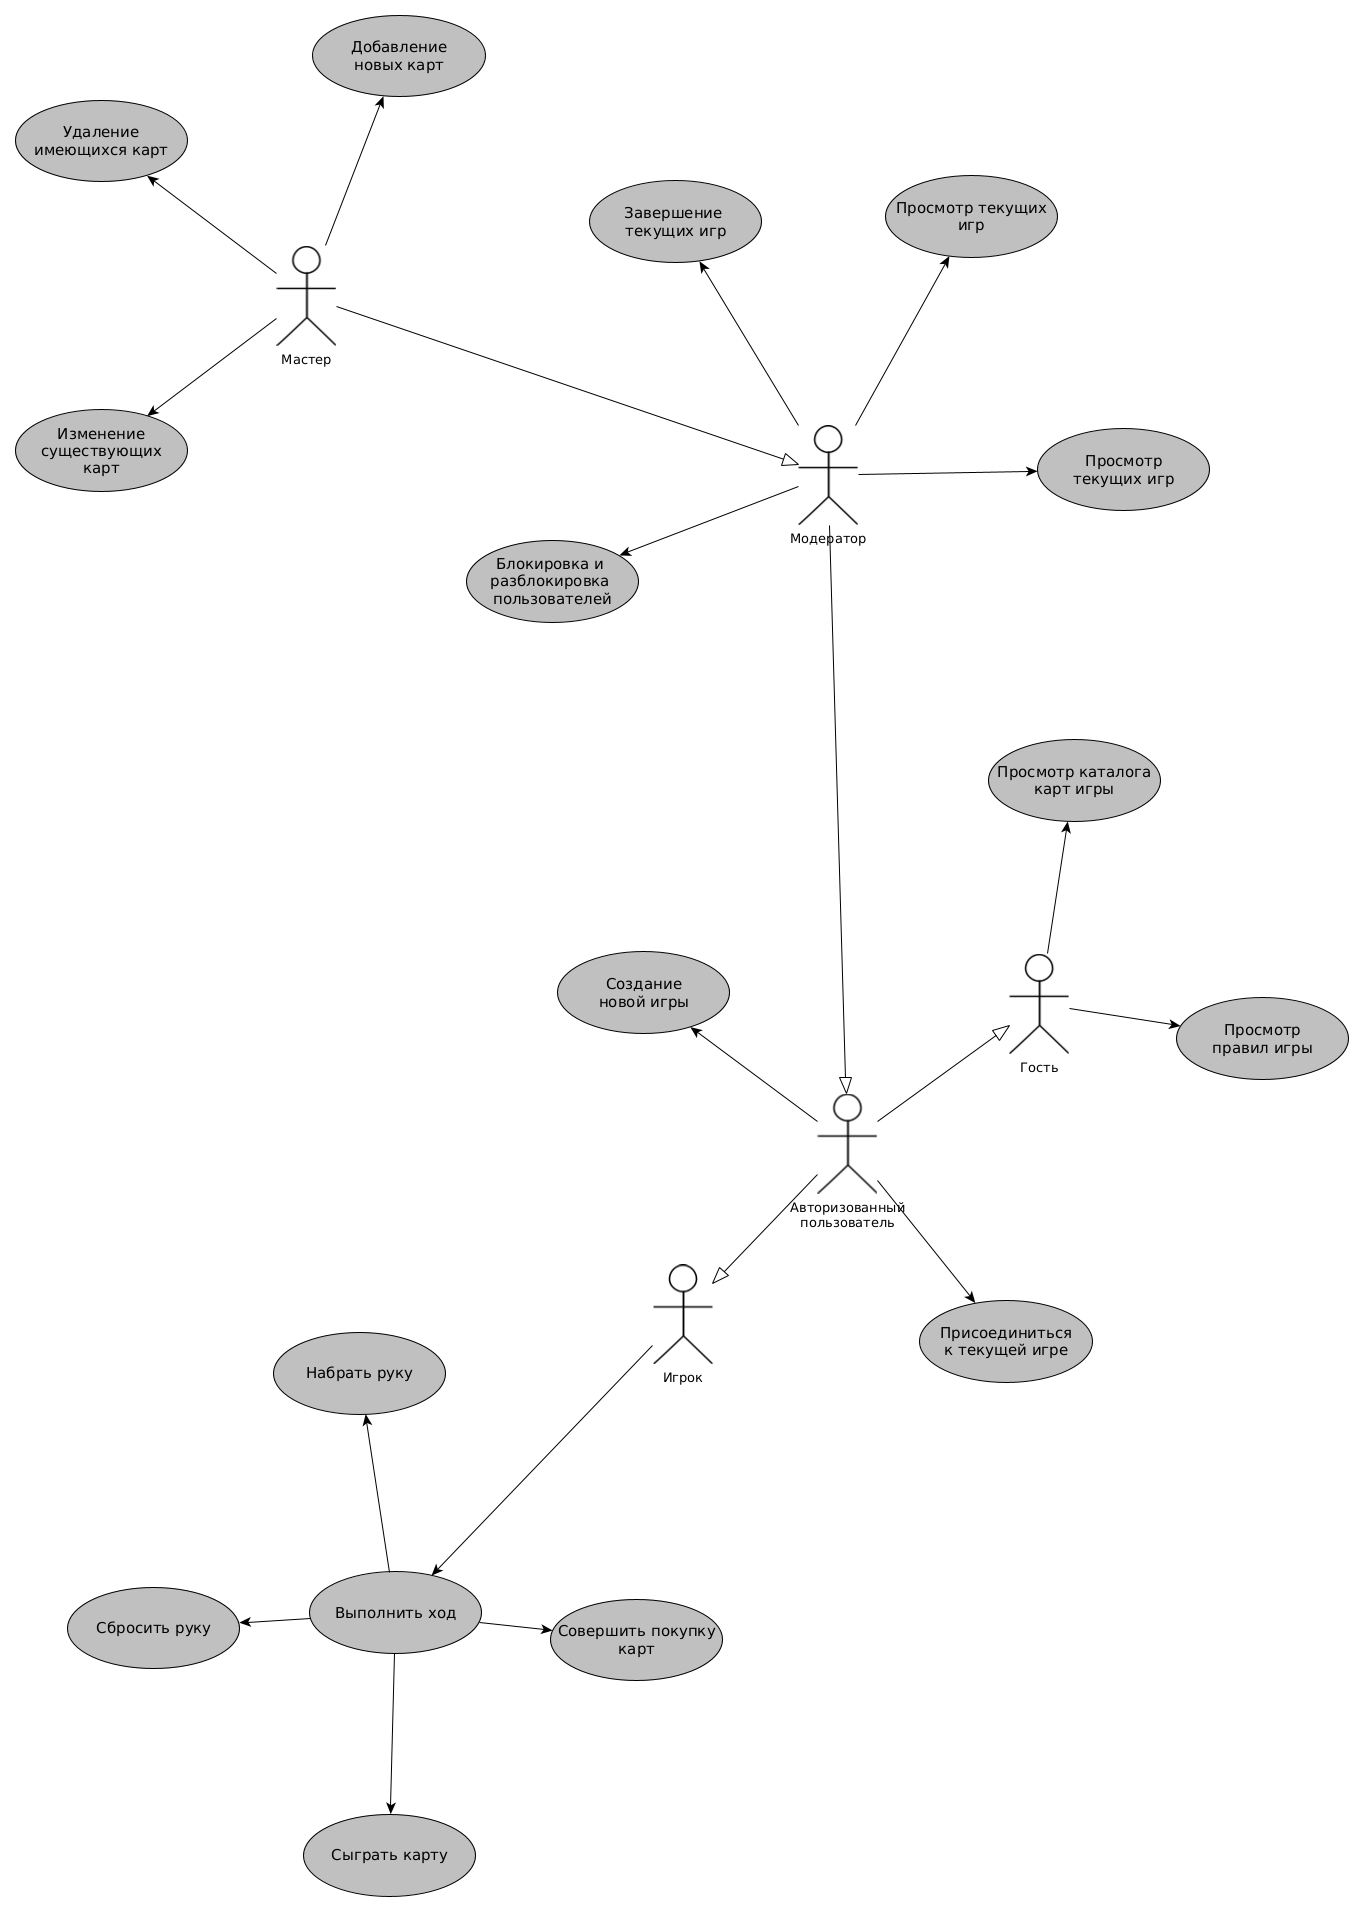
\includegraphics[width=1\linewidth]{../img/r-use-case}
	\caption{Диаграмма вариантов использования разрабатываемой системы}
	\label{img:r-use-case}
\end{figure}

\section{Требования к разрабатываемому приложению}
Разрабатываемый сайт предназначен для одного или нескольких гостей, способных
просматривать игровые карты и правила игры, и пользователей, способных
авторизоваться и быть участниками игровых партий.

Таким образом, разрабатываемое приложение должно обладать следующей
функциональностью:
\begin{enumerate}
	\item управление игровыми сессиями (создание, подключение и завершение
	      игры);
	\item взаимодействие игроков в рамках игровой сессии;
	\item отображение текущего состояния игры (поле, карты, колоды и прочие
	      игровые сущности);
	\item выполнение игровых действий пользователем (применение эффектов
	      карт,
	      покупка новых);
	\item обработка логики игры (подсчёт очков, применение правил, переходы
	      между состояниями);
	\item поддержка работы с колодами карт (формирование, перемешивание,
	      добор
	      и сброс карт);
\end{enumerate}

Таким образом, приложение должно обеспечивать полный цикл управления игровыми
сессиями, включая создание, участие в игре и просмотр результатов.

\section{Формализация данных}

В таблице~\ref{tbl:data} представлены сущности, используемые в базе данных.

\begin{longtable}{|>{\raggedright\arraybackslash}p{0.14\textwidth}|>{\raggedright\arraybackslash}p{0.14\textwidth}|>{\raggedright\arraybackslash}p{0.26\textwidth}|>{\raggedright\arraybackslash}p{0.12\textwidth}|>{\raggedright\arraybackslash}p{0.14\textwidth}|}
	\caption{Сущности и их свойства} \label{tbl:data}
	\\
	\hline
	\textbf{Сущность} & \textbf{Свойство} & \textbf{Метка}
	                  & \textbf{Тип}      &
	\textbf{Атрибут БД}
	\\
	\hline
	\endfirsthead
	\caption{Сущности и их свойства}
	\\
	\hline
	\textbf{Сущность} & \textbf{Свойство} & \textbf{Метка}
	                  & \textbf{Тип}      & \textbf{Атрибут БД}
	\\
	\hline
	\endhead
	\hline
	\endfoot
	\endlastfoot

	\textbf{Пользо-\newline ватель}
	                  & Псевдоним         & Имя пользователя, уникально
	                  & Строка            & \texttt{username}
	\\
	\cline{2-5}
	                  & Эл. почта         & Адрес почты, уникально
	                  & Строка            & \texttt{e-mail}
	\\
	\cline{2-5}
	                  & Пароль            & Хеш пароля
	                  & Строка            & \texttt{password}
	\\
	\cline{2-5}
	                  & Дата рег.         & Время создания аккаунта
	                  & DateTime          &
	\texttt{register\_\newline date}
	\\
	\hline

	\textbf{Игра}
	                  & Текущий ход       & Номер текущего хода
	                  & Целое число       &
	\texttt{current\_move}
	\\
	\cline{2-5}
	                  & Памятки           & Оставшееся кол-во памяток
	                  & Целое число       & \texttt{memos}
	\\
	\cline{2-5}
	                  & Время начала      & Момент старта партии
	                  & DateTime          & \texttt{time\_start}
	\\
	\cline{2-5}
	                  & Победитель        & Внешний ключ к Players, может
	быть NULL         & Целое число       &
	\texttt{winner}
	\\
	\hline

	\textbf{Игрок}
	                  & Пользователь      & Внешний ключ к Users
	                  & Целое число       & \texttt{user\_id}
	\\
	\cline{2-5}
	                  & Игра              & Внешний ключ к Games
	                  & Целое число       & \texttt{game\_id}
	\\
	\cline{2-5}
	                  & Здоровье          & Текущее здоровье
	                  & Целое число       & \texttt{health}
	\\
	\cline{2-5}
	                  & Лимит руки        & Макс. карт в руке
	                  & Целое число       & \texttt{hand\_limit}
	\\
	\cline{2-5}
	                  & Базовое эхо       & Базовый ресурс
	                  & Целое число       & \texttt{base\_echo}
	\\
	\cline{2-5}
	                  & Порядок хода      & Очередность хода игрока
	                  & Целое число       & \texttt{turn}
	\\
	\hline

	\textbf{Карта}
	                  & Название          & Название карты
	                  & Строка            & \texttt{title}
	\\
	\cline{2-5}
	                  & Эхо               & Количество эхо карты
	                  & Целое число       & \texttt{echo}
	\\
	\cline{2-5}
	                  & Стоимость         & Цена покупки
	                  & Целое число       & \texttt{cost}
	\\
	\cline{2-5}
	                  & Сила              & Значение эффекта
	                  & Целое число       & \texttt{power}
	\\
	\cline{2-5}
	                  & Тип карты         & Внешний ключ к Types
	                  & Целое число       & \texttt{card\_type}
	\\
	\cline{2-5}
	                  & Очки крутости     & Очки за карту
	                  & Целое число       & \texttt{cool\_points}
	\\
	\hline

	\textbf{Тип карты}
	                  & Действие          & Тип эффекта
	                  & Строка            & \texttt{action}
	\\
	\cline{2-5}
	                  & Постоянность      & Признак постоянного эффекта
	                  & Логический        &
	\texttt{if\_permanent}
	\\
	\hline

	\textbf{Колода}
	                  & Тип               & Тип (market, hand и т.д.)
	                  & Строка            & \texttt{type}
	\\
	\cline{2-5}
	                  & Открытость        & Могут карты быть просмотрены
	или нет           & Логический        &
	\texttt{if\_open}
	\\
	\cline{2-5}
	                  & Владелец          & Внешний ключ к Players, может
	быть NULL         & Целое число       &
	\texttt{owner\_id}
	\\
	\hline

	\textbf{Карта в колоде}
	                  & Колода            & Внешний ключ к Decks
	                  & Целое число       & \texttt{deck\_id}
	\\
	\cline{2-5}
	                  & Карта             & Внешний ключ к Cards
	                  & Целое число       & \texttt{card\_id}
	\\
	\cline{2-5}
	                  & Позиция           & Порядковый номер карты в
	стопке            & Целое число       &
	\texttt{position}
	\\
	\hline

	\textbf{Изображение}
	                  & Название          & Имя файла/заголовка
	                  & Строка            & \texttt{title}
	\\
	\cline{2-5}
	                  & Файл              & Путь к файлу изображения
	                  & Path              & \texttt{file}
	\\
	\hline
\end{longtable}

На рисунке~\ref{img:er} представлена диаграмма сущность-связь, отражающая
структуру базы данных и связи между сущностями.

\begin{figure}[H]
	\centering
	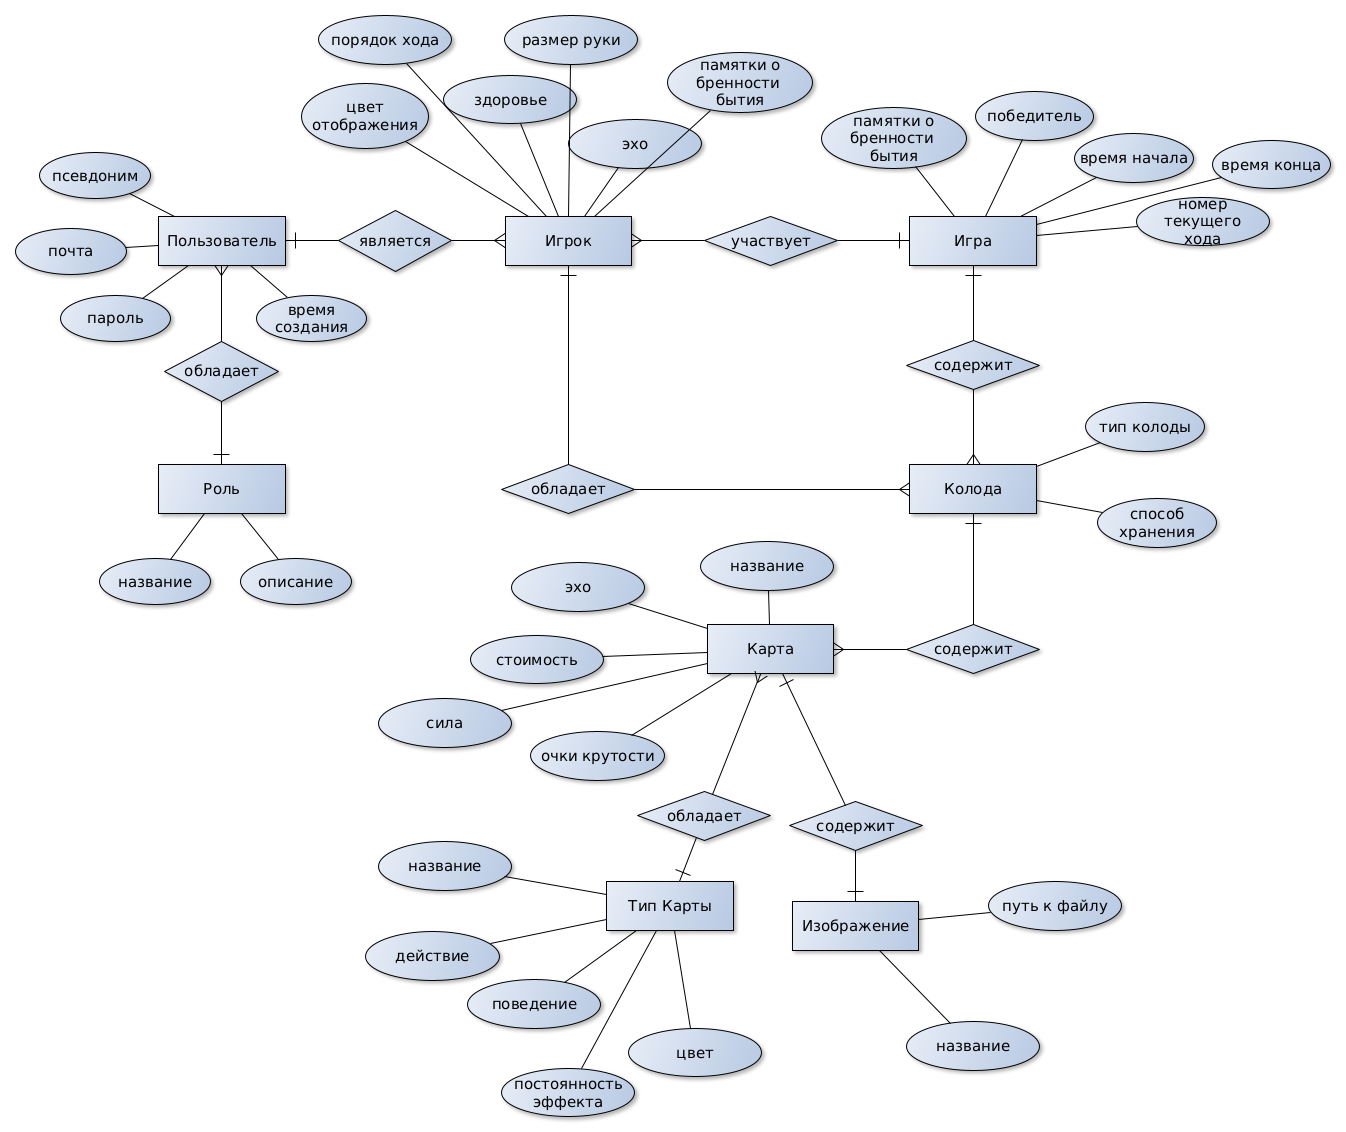
\includegraphics[width=1\linewidth]{../img/er.png}
	\caption{Диаграмма сущность-связь в нотации Чена}
	\label{img:er}
\end{figure}

\section{Выбор модели хранения данных}

В разрабатываемой системе предполагается хранение структурированных данных
предметной области, включающих сущности (например, пользователи, игровые
объекты, карты) и связи между ними. Для каждой сущности задан фиксированный
набор атрибутов и предусмотрены взаимосвязи, требующие поддержания целостности
и согласованности данных~\cite{lectures}.

Существует несколько основных моделей хранения данных:

\begin{description}
	\item[Дореляционная модель] --- данные хранятся в виде иерархических
		структур, файлов или сетевых баз данных. Эта модель не
		предполагает жёсткой
		схемы таблиц и характеризуется сложностью в обеспечении
		ссылочной целостности.
		Операции с данными требуют специализированного программного
		обеспечения, а
		структура данных тесно связана с применением. Дореляционный
		подход хорошо
		подходит для специализированных приложений, но неудобен для
		систем, требующих
		гибкости и универсальности~\cite{lectures}.

	\item[Реляционная модель] --- информация представляется в виде таблиц с
		явно определёнными атрибутами, первичными и внешними ключами,
		ограничениями
		целостности и уникальности. Реляционная модель обеспечивает
		строгое разделение
		структуры данных от логики приложения, позволяет использовать
		стандартный язык
		запросов (SQL), удобна для сложных операций и обеспечивает
		надёжность данных
		через механизмы транзакций~\cite{date}.

	\item[Постреляционная модель] --- Такие БД основаны на реляционных,
		однако
		отходят от их принципов в пользу более эффективного решения
		специфических
		задач. Одним из примеров таких особенностей выступает
		возможность вложенного
		хранения таблиц (хранения таблиц в таблицах), что невозможно в
		реляционных
		БД~\cite{postrel}.
\end{description}

С учётом требований разрабатываемой системы наиболее подходящей является
реляционная модель данных. Она позволяет явно определить структуру данных
(пользователи, игры, игроки, карты, колоды), обеспечить строгое соблюдение
ограничений целостности, поддержать сложные многотабличные запросы для анализа
состояния игры и гарантировать консистентность данных при одновременном доступе
нескольких игроков. Реляционная модель удобна для выполнения сложных запросов и
фильтрации информации.

\section*{Вывод}

В аналитической части была рассмотрена предметная область, были рассмотрены и
формализованы данные, подлежащие хранению и выбрана реляционная модель хранения
данных.
\include{latex-parts/05-design_part}
\chapter{Технологический раздел}
В рамках технологической части были выбраны средства реализации проекта,
описаны программы для создания и запуска базы данных, триггера валидации карты
и
хранимой процедуры проверки покупки, описанных в конструкторской части. Был
описан алгоритм тестирования разработанных триггера и процедуры.

\section{Средства реализации}
В качестве СУБД был выбран Postgresql~\cite{postgres} так как он позволяет
реализовать разработанную структуру данных и ролевую модель, а также
поддерживает реализацию триггеров на добавление и обновление данных.

Для хранения файлов, в частности изображений карт, было выбрано объектное
хранилище Minio~\cite{minio} так как оно позволяет легко и быстро развернуть
хранилище объектов, независимое от файловой и операционной системы.

\section{Создание базы данных}

В качестве языка основного языка для написания проекта был выбран
Python~\cite{python} так как средств языка достаточно для разработки
приложения, есть библиотеки для взаимодействия с Postgresql~\cite{psycorg2} и
Minio~\cite{minio-python}.

\section{Создание базы данных}

На основе разработанной в конструкторском разделе реляционной схемы были
реализованы таблицы пользователей, партий, игроков, карт, типов карт,
изображений, колод и карт в колодах. В программе создания базы данных задаются
первичные и внешние ключи, ограничения уникальности, обязательность полей и
связи между таблицами.

Создание базы данных происходит в два этапа. На первом этапе создаётся схема
базы данных и накладываются ограничения целостности. Для этого используются
миграции Alembic~\cite{alembic}, которые формируют и последовательно применяют
SQL-команды создания и изменения таблиц. Скрипт представлен в приложении А в
листинге~\ref{lst:alembic}.

На втором этапе база данных заполняется начальными данными: типами карт,
изображениями и набором игровых карт. Этап заполнения базы данных представлен в
листинге~\ref{lst:fill_db}.

Интерфейс доступа к базе данных реализован через репозитории пользователей,
карт, типов карт и партий. Репозитории используют сессии SQLAlchemy,
создаваемые фабрикой \texttt{SessionFactory}, поэтому прикладная логика
обращается к базе данных через методы предметного уровня, а не через
SQL-запросы напрямую.

\section{Роли и их права}
В конструкторской части были выделены следующие пять ролей:
\begin{itemize}
	\item пользователь (гость);
	\item авторизованный пользователь;
	\item игрок;
	\item модератор;
	\item мастер.
\end{itemize}

Кроме стандартных прав на уровне ролей, для дополнительной защиты данных
использовалась фильтрация строк PostgreSQL \texttt{postgres-rls}, которая
ограничивает доступ к записям в таблицах на уровне строк.

Код для создания ролей и определения прав доступа представлен в приложении А в
листингах~\ref{lst:user-role}~---~\ref{lst:master-role}.

\section{Триггер валидации карты}

Для обеспечения целостности данных был разработан триггер, который при каждом
вставлении или обновлении записи в таблице \texttt{cards} проверяет
соответствие характеристик карты установленным ограничениям. Если одно из
условий не выполняется, триггер прерывает операцию и откатывает изменение.
Код разработанного триггера представлен в приложении А, в
листинге~\ref{lst:card_check_trigger}.

\section{Процедура проверки покупки}

Для проверки покупки карты была реализована хранимая процедура, которая
проверяет доступность карты, текущее эхо игрока и бизнес-правила перед
совершением покупки. Если объём эхо меньше стоимости карты, процедура
генерирует исключение, и операция покупки не выполняется.
Код хранимой процедуры представлен в приложении А, в
листинге~\ref{lst:card_buy_procedure}.

\section{Redis (кэширование)}

Для повышения производительности системы при работе с каталогом карт
используется Redis~\cite{redis}, его применение позволяет сократить количество
обращений к базе данных.

В кэше сохраняются готовые JSON-ответы для эндпоинтов, предназначенных только
для просмотра данных каталога карт. При поступлении запроса система сначала
проверяет наличие соответствующих данных в Redis. Если данные найдены, ответ
формируется непосредственно из кэша, в противном
случае информация извлекается из базы данных, преобразуется в
JSON-представление и сохраняется в Redis для последующих запросов.

Для обеспечения актуальности данных каждой записи в кэше назначается
ограниченное время жизни (TTL, Time To Live). После истечения этого времени
запись автоматически удаляется из Redis и при следующем обращении формируется
заново на основе данных из базы данных.

При добавлении, изменении или удалении карты записи кэша, связанные с каталогом
карт, принудительно удаляются.

\section{Пользовательский интерфейс}

В качестве пользовательского интерфейса было разработано веб-приложение с
игрой, предоставляющее описанную в аналитической части функциональность.
Приложение разделено на основные компоненты, представляющие различные этапы
взаимодействия пользователя с системой: авторизация, просмотр каталога карт,
редактирование колод и процесс игровой сессии. Описание компонентов
пользовательского интерфейса представлено в UML формате на
рисунке~\ref{img:ui-uml}.

\begin{figure}[H]
	\centering
	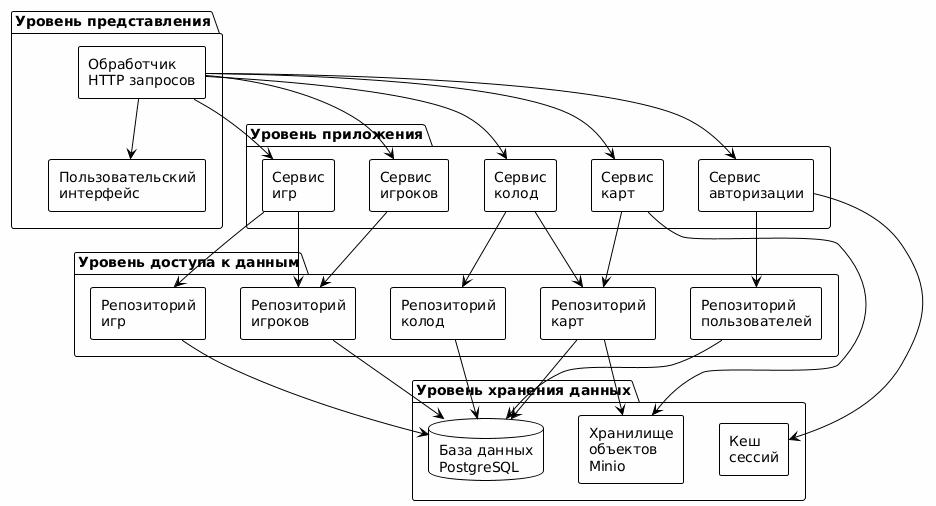
\includegraphics[width=0.9\linewidth]{../img/ui-uml}
	\caption{Диаграмма компонентов пользовательского интерфейса}
	\label{img:ui-uml}
\end{figure}

\section{Тестирование}

\subsection{Тестирование приложения}

Модульное тестирование приложения проводилось с помощью фреймворка
\texttt{pytest}~\cite{pytest} и стандартной библиотеки
\texttt{unittest.mock} для изоляции тестируемых компонентов.

Тестами были покрыты модули игровой логики, логики карт, управления
состоянием партии, сервиса колод и контроля доступа.

Покрытие кода составило 84\%.

\subsection{Тестирование триггера валидации карты}

Тестирование триггера проводилось с помощью тестов на языке Python.
Были выделены следующие классы эквивалентности:

\begin{itemize}
	\item корректная карта (все поля в допустимых пределах);
	\item карта с нулевой стоимостью (\texttt{cost} = 0);
	\item карта со стоимостью выше максимума (\texttt{cost} > 7);
	\item карта с нулевой силой (\texttt{power} = 0);
	\item карта типа \texttt{buff\_*} с силой выше 2 (\texttt{power} > 2);
	\item карта с \texttt{cool\_points} ниже минимума (< $-1$);
	\item карта с \texttt{cool\_points} выше максимума (> 5);
	\item карта без типа (\texttt{card\_type\_id} = NULL);
	\item карта типа \texttt{buff\_*} с пустым полем \texttt{creature};
	\item карта типа \texttt{buff\_*} с непустым полем \texttt{creature}.
\end{itemize}

Каждый класс эквивалентности был протестирован на операциях вставки
и обновления. Общий алгоритм тестирования триггера имел следующий вид:

\begin{enumerate}
	\item Создание тестовых данных в базе данных (тип карты, изображение).
	\item Цикл по всем тестам:
	      \begin{enumerate}
		      \item вставка записи карты с тестовыми данными;
		      \item если тест позитивный:
		            \begin{itemize}
			            \item проверка, что триггер не вызвал
			                  ошибку;
			            \item проверка, что запись успешно
			                  добавлена в таблицу;
		            \end{itemize}
		      \item иначе:
		            \begin{itemize}
			            \item проверка, что триггер вызвал ошибку;
			            \item проверка, что запись не добавлена в
			                  базу данных;
		            \end{itemize}
		      \item очистка таблицы карт.
	      \end{enumerate}
	\item Цикл по всем тестам:
	      \begin{enumerate}
		      \item создание корректной записи карты;
		      \item обновление записи согласно тестовым данным;
		      \item если тест позитивный:
		            \begin{itemize}
			            \item проверка, что триггер не вызвал
			                  ошибку;
			            \item проверка, что запись успешно
			                  изменена;
		            \end{itemize}
		      \item иначе:
		            \begin{itemize}
			            \item проверка, что триггер вызвал ошибку;
			            \item проверка, что запись не изменена.
		            \end{itemize}
	      \end{enumerate}
\end{enumerate}

\subsection{Тестирование процедуры проверки покупки}

Тестирование хранимой процедуры проводилось с помощью тестов на языке Python.
Были выделены следующие классы эквивалентности:

\begin{itemize}
	\item корректная покупка при достаточном количестве эхо;
	\item покупка при недостаточном количестве эхо;
	\item покупка несуществующей карты;
	\item покупка карты, которой нет в каталоге.
\end{itemize}

Общий алгоритм тестирования процедуры имел следующий вид:

\begin{enumerate}
	\item Создание тестовых данных: игрока с заданным количеством эхо и
	      карты с заданной стоимостью.
	\item Вызов процедуры с тестовыми параметрами.
	\item Если тест позитивный:
	      \begin{itemize}
		      \item проверка, что процедура не вызвала исключение;
		      \item проверка, что стоимость карты вычтена из баланса
		            эхо
		            игрока;
		      \item проверка, что карта добавлена в колоду игрока.
	      \end{itemize}
	\item Иначе:
	      \begin{itemize}
		      \item проверка, что процедура вызвала исключение;
		      \item проверка, что баланс эхо игрока не изменился;
		      \item проверка, что карта не добавлена в колоду игрока.
	      \end{itemize}
\end{enumerate}

\section*{Вывод}
В результате технологической части были выбраны средства реализации работы,
созданы
база данных, роли, триггер и хранимая процедура. Также было разработано и
протестировано приложение для игры.
\chapter{Исследовательский раздел}

\section{Цель исследования}

Целью исследования является анализ влияния размера личной колоды игрока и
используемой структуры хранения данных на производительность операций
завершения хода и формирования новой руки игрока.

В рамках исследования сравнивались структуры данных
\texttt{list}~\cite{py-list} и
\texttt{deque}~\cite{py-deque},
используемые для хранения игровых колод. Также оценивалось влияние
необходимости
перемешивания сброса на общее время выполнения операций.

\section{Методика проведения исследования}

Для проведения исследования была реализована программа, моделирующая завершение
хода игрока.

Во время выполнения операции выполнялись следующие шаги:

\begin{enumerate}
	\item перенос карт из руки игрока в сброс;
	\item перенос карт из сброса обратно в колоду добора;
	\item перемешивание колоды;
	\item добор новой руки.
\end{enumerate}

Исследование проводилось для двух вариантов организации хранения колоды:

\begin{itemize}
	\item \texttt{list};
	\item \texttt{deque}.
\end{itemize}

Замеры выполнялись для колод различных размеров:

\begin{itemize}
	\item 20 карт;
	\item 50 карт;
	\item 100 карт;
	\item 200 карт;
	\item 500 карт;
	\item 1000 карт;
	\item 2000 карт.
\end{itemize}

Для уменьшения влияния случайных факторов каждый эксперимент повторялся 1000
раз, после чего вычислялось среднее время выполнения операции.

Дополнительно исследования выполнялись в двух режимах:

\begin{itemize}
	\item без перемешивания сброса;
	\item с перемешиванием сброса.
\end{itemize}

Время выполнения измерялось с использованием функции \texttt{perf\_counter()}
языка Python.

\section{Результаты исследования}

В ходе исследования были построены графики зависимости времени выполнения
операции завершения хода от размера колоды. Графики представлены на
рисунках~\ref{img:full},~\ref{img:small}.

\begin{figure}[H]
	\centering
	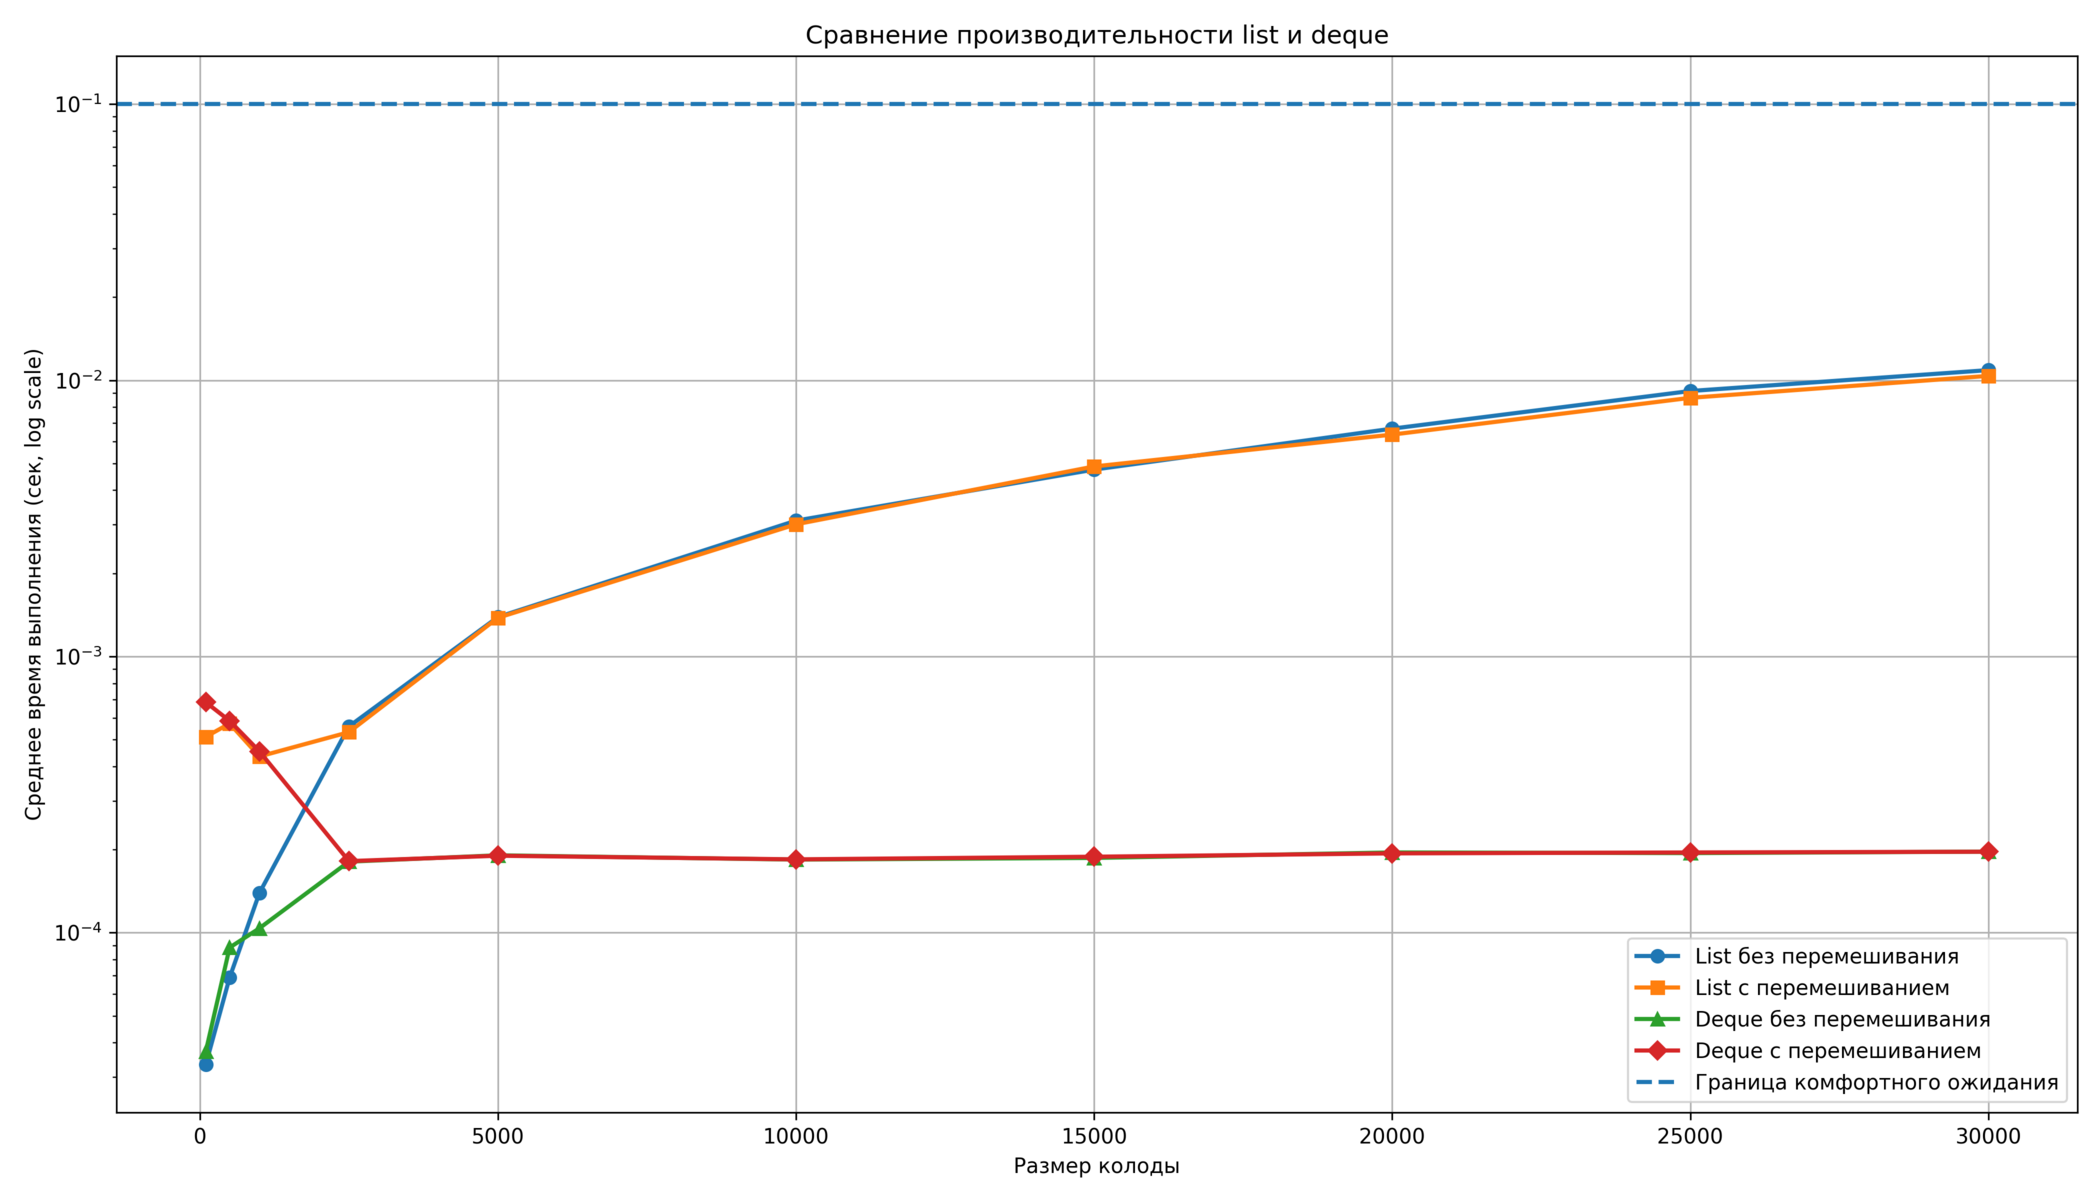
\includegraphics[width=0.9\linewidth]{../img/deck_performance_full}
	\caption{График замеров времени формирования колоды с временем
		комфортного ожидания пользователя}
	\label{img:full}
\end{figure}

\begin{figure}[H]
	\centering
	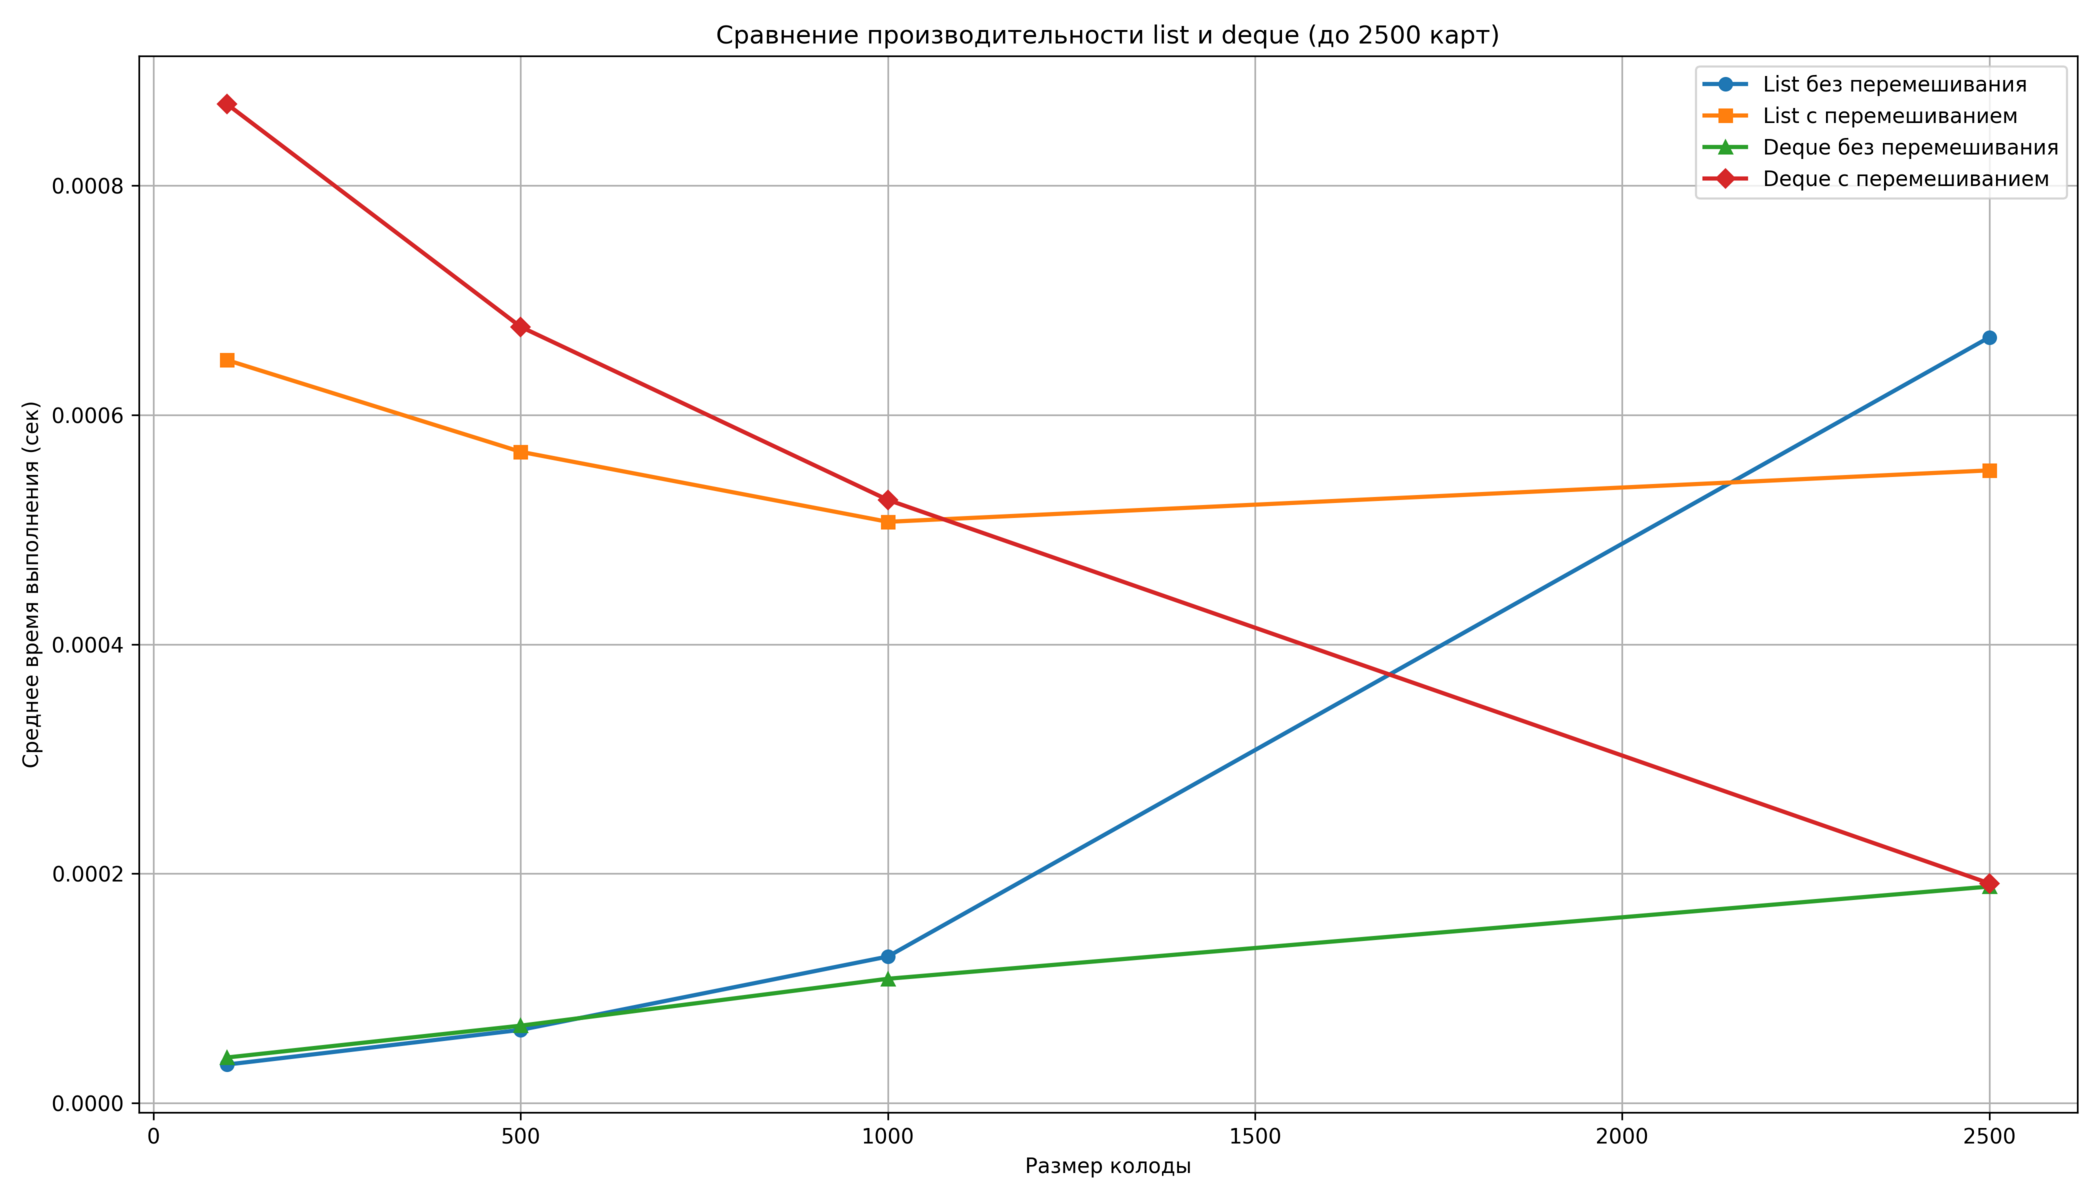
\includegraphics[width=0.9\linewidth]{../img/deck_performance_small}
	\caption{График замеров времени формирования колоды на малых значениях}
	\label{img:small}
\end{figure}

Результаты показали, что:

\begin{itemize}
	\item время выполнения операций увеличивается с ростом размера колоды;
	\item необходимость перемешивания оказывает значительно большее влияние
	      на
	      производительность, чем сам размер колоды;
	\item структура \texttt{list} демонстрирует более высокую
	      производительность при
	      отсутствии перемешивания;
	\item при использовании перемешивания различия между \texttt{list} и
	      \texttt{deque}
	      уменьшаются из-за дополнительных затрат на перестановку
	      элементов.
\end{itemize}

Также было установлено, что основное время выполнения затрачивается на операции
копирования и перемешивания элементов колоды.

\section*{Вывод}

В результате исследования было установлено, что производительность игровых
операций зависит не только от размера колоды, но и от используемой структуры
хранения данных, а также от необходимости перемешивания сброса.

Для операций последовательного хранения и добора карт структура \texttt{list}
показала более высокую производительность. Однако при частых операциях удаления
элементов из начала коллекции использование \texttt{deque} позволяет уменьшить
накладные расходы.

Наибольшее влияние на время выполнения оказывает операция перемешивания колоды,
поскольку она требует обработки всех элементов коллекции.

\include{latex-parts/10-role_based_access}
\ssr{ЗАКЛЮЧЕНИЕ}

В результате курсовой работы был проведён анализ предметной области настольной
игры <<Эпичные схватки боевых магов: Крутагидон>>. Были формализованы данные о
пользователях, партиях, картах, колодах, выделены роли пользователей и их
сценарии использования.

Была спроектирована реляционная база данных, для хранения данных о
пользователях, играх, игроках, картах и колодах, описаны ограничения
целостности,
сформулированы ограничения доступа и действий каждой роли в системе.

В результате работы был разработан сайт для игры в онлайн-версию <<Эпичных
схваток боевых магов: Крутагидон>>.
Разработанное ПО позволяет создавать новые игры и присоединяться к уже
существующим, управлять колодами карт, просматривать информацию о картах и
игроках, а также выполнять игровые действия в рамках партий.

В ходе исследования была проведена проверка корректности работы разработанной
системы и основных игровых операций. Были протестированы механики покупки и
розыгрыша карт, перехода хода между игроками, работы игровых колод, а также
ограничения целостности базы данных, триггеры и хранимые процедуры. Результаты
исследования показали корректную работу реализованной игровой логики и
соответствие системы сформулированным требованиям.

В ходе работы поставленные цель и задачи были выполнены.

\def\bibname{\begin{center}\vspace{-1.3cm} \Large СПИСОК ИСПОЛЬЗОВАННЫХ
        ИСТОЧНИКОВ\end{center}}
\addcontentsline{toc}{chapter}{СПИСОК ИСПОЛЬЗОВАННЫХ ИСТОЧНИКОВ}
\begin{thebibliography}{}
	\bibitem{rules} Мосигра. Правила игры <<Эпичные схватки боевых магов.
	Крутагидон>> // URL:

	\url{https://www.mosigra.ru/download/rules/jepichnie-shvatki-boevih-magov-krutagidon-2025-rules.pdf}
	(дата обращения: 20.02.2026).
	\bibitem{lectures} Конспекты лекций курса <<Базы данных>> за 2024 год.
	МГТУ им. Н.Э. Баумана, кафедра <<Программное обеспечение ЭВМ и
	информационные
	технологии>>. Учебные материалы.
	\bibitem{date} Дейт К. Дж. Введение в системы баз данных. --- 8-е изд.
	--- М.: Издательский дом ``Вильяме'', 2005. --- 1328 с.
	\bibitem{postrel} Парфенов, Ю. П. Постреляционные хранилища данных :
	учеб. пособие. --- Екатеринбург: изд-во Урал, 2016. --- 120 с.
	\bibitem{postgres} PostgreSQL: The World's Most Advanced Open Source
	Relational Database // URL: \url{https://www.postgresql.org/} (дата
	обращения:
	01.05.2026).
	\bibitem{minio} MinIO: High Performance Data Store for AI \& Analytics
	// URL: \url{https://www.min.io/} (дата обращения: 01.05.2026).
	\bibitem{python} Python: The Programming Language // URL:
	\url{https://www.python.org/} (дата обращения: 01.05.2026).
	\bibitem{psycorg2} Psycopg2: Python interface to PostgreSQL // URL:
	\url{https://www.psycopg.org/} (дата обращения: 01.05.2026).
	\bibitem{minio-python} Minio Python Client Library // URL:
	\url{https://docs.min.io/docs/python-client-api-reference.html} (дата
	обращения: 01.05.2026).
	\bibitem{alembic} Alembic: Database Migrations for SQLAlchemy // URL:
	\url{https://alembic.sqlalchemy.org/} (дата обращения: 01.05.2026).
	\bibitem{postgres-rls} Row Level Security in PostgreSQL // URL:
	\url{https://www.postgresql.org/docs/current/ddl-rowsecurity.html}
	(дата
	обращения: 01.05.2026).
	\bibitem{py-list} More on Lists // Python Documentation URL:

	\url{https://docs.python.org/3/tutorial/datastructures.html#more-on-lists}
	(дата обращения: 01.05.2026).
	\bibitem{py-deque} Container datatypes // Python Documentation URL:

	\url{https://docs.python.org/3/library/collections.html#collections.deque}
	(дата обращения: 01.05.2026).

	\bibitem{redis} Redis // Real-time data for agents \& apps URL:
	\url{https://redis.io/} (дата обращения: 01.05.2026).
\end{thebibliography}
\ssr{Приложение A}

\begin{lstlisting}[language=Python, caption={Скрипт миграции Alembic},
			label={lst:alembic}]
	from collections.abc import Sequence
	from uuid import UUID

	import sqlalchemy as sa
	from alembic import op
	from sqlalchemy.dialects import postgresql

	revision: str = "001_initial"
	down_revision: str | None = None
	branch_labels: str | Sequence[str] | None = None
	depends_on: str | Sequence[str] | None = None

	DEFAULT_CARD_TYPE_ID = UUID("6c9097de-cd28-5eab-975b-8a7de384fd6f")


	def upgrade() -> None:
		op.create_table(
			"users",
			sa.Column("id", postgresql.UUID(as_uuid=True), nullable=False),
			sa.Column("username", sa.String(length=50), nullable=False),
			sa.PrimaryKeyConstraint("id"),
			sa.UniqueConstraint("username", name="uq_user_username"),
		)

		op.create_table(
			"card_types",
			sa.Column("id", postgresql.UUID(as_uuid=True), nullable=False),
			sa.Column("action", sa.String(length=50), nullable=False),
			sa.Column("usage_pattern", sa.String(length=50), nullable=False),
			sa.Column("if_permanent", sa.Boolean(), nullable=False, server_default="false"),
			sa.Column("color", sa.String(length=50), nullable=False, server_default="red"),
			sa.PrimaryKeyConstraint("id"),
		)

		op.execute(
			sa.text(
				"""
				INSERT INTO card_types (id, action, usage_pattern, if_permanent, color)
				VALUES (:card_type_id, 'attack', 'reg', false, 'red')
				ON CONFLICT (id) DO NOTHING
				"""
			).bindparams(
				sa.bindparam(
					"card_type_id",
					value=DEFAULT_CARD_TYPE_ID,
					type_=postgresql.UUID(as_uuid=True),
				)
			)
		)

		op.create_table(
			"games",
			sa.Column("id", postgresql.UUID(as_uuid=True), nullable=False),
			sa.Column("host_user_id", postgresql.UUID(as_uuid=True), nullable=False),
			sa.Column("status", sa.String(length=50), nullable=False),
			sa.Column("cur_turn", sa.Integer(), nullable=False, server_default="0"),
			sa.Column("cur_player_id", postgresql.UUID(as_uuid=True), nullable=True),
			sa.Column("winner_id", postgresql.UUID(as_uuid=True), nullable=True),
			sa.ForeignKeyConstraint(["host_user_id"], ["users.id"]),
			sa.PrimaryKeyConstraint("id"),
		)

		# images table: stores image metadata for cards
		op.create_table(
			"images",
			sa.Column("id", postgresql.UUID(as_uuid=True), nullable=False),
			sa.Column("title", sa.String(length=200), nullable=False),
			sa.Column("file", sa.String(length=500), nullable=True),
			sa.PrimaryKeyConstraint("id"),
		)

		op.create_table(
			"cards",
			sa.Column("id", postgresql.UUID(as_uuid=True), nullable=False),
			sa.Column("title", sa.String(length=200), nullable=False),
			sa.Column("creature", sa.String(length=100), nullable=False),
			sa.Column("power", sa.Integer(), nullable=False, server_default="2"),
			sa.Column("echo", sa.Integer(), nullable=False, server_default="1"),
			sa.Column("cost", sa.Integer(), nullable=False, server_default="3"),
			sa.Column("cool_points", sa.Integer(), nullable=False, server_default="0"),
			sa.Column(
				"card_type_id",
				postgresql.UUID(as_uuid=True),
				nullable=False,
				server_default=str(DEFAULT_CARD_TYPE_ID),
			),
			sa.Column(
				"image_id",
				postgresql.UUID(as_uuid=True),
				nullable=False,
			),
			sa.ForeignKeyConstraint(["card_type_id"], ["card_types.id"]),
			sa.ForeignKeyConstraint(["image_id"], ["images.id"]),
			sa.PrimaryKeyConstraint("id"),
			sa.UniqueConstraint("title", name="uq_cards_title"),
		)

		op.alter_column("cards", "card_type_id", server_default=None)

		op.create_table(
			"players",
			sa.Column("id", postgresql.UUID(as_uuid=True), nullable=False),
			sa.Column("game_id", postgresql.UUID(as_uuid=True), nullable=False),
			sa.Column("user_id", postgresql.UUID(as_uuid=True), nullable=False),
			sa.Column("nickname", sa.String(length=50), nullable=False),
			sa.Column("turn_order", sa.Integer(), nullable=False, server_default="0"),
			sa.Column("health", sa.Integer(), nullable=False, server_default="20"),
			sa.Column("base_echo", sa.Integer(), nullable=False, server_default="0"),
			sa.Column("cur_echo", sa.Integer(), nullable=False, server_default="0"),
			sa.Column("hand_size", sa.Integer(), nullable=False, server_default="5"),
			sa.ForeignKeyConstraint(["game_id"], ["games.id"], ondelete="CASCADE"),
			sa.ForeignKeyConstraint(["user_id"], ["users.id"]),
			sa.PrimaryKeyConstraint("id"),
			sa.UniqueConstraint("game_id", "user_id", name="uq_players_game_user"),
		)

		op.create_foreign_key(
			"fk_games_winner_id_players",
			"games",
			"players",
			["winner_id"],
			["id"],
		)

		op.create_table(
			"decks",
			sa.Column("id", postgresql.UUID(as_uuid=True), nullable=False),
			sa.Column("type", sa.String(length=50), nullable=False),
			sa.Column("game_id", postgresql.UUID(as_uuid=True), nullable=True),
			sa.Column("player_id", postgresql.UUID(as_uuid=True), nullable=True),
			sa.Column("if_open", sa.Boolean(), nullable=False, server_default="false"),
			sa.ForeignKeyConstraint(["game_id"], ["games.id"]),
			sa.ForeignKeyConstraint(["player_id"], ["players.id"]),
			sa.PrimaryKeyConstraint("id"),
		)

		op.create_table(
			"deck_cards",
			sa.Column("id", postgresql.UUID(as_uuid=True), nullable=False),
			sa.Column("deck_id", postgresql.UUID(as_uuid=True), nullable=False),
			sa.Column("card_id", postgresql.UUID(as_uuid=True), nullable=False),
			sa.Column("position", sa.Integer(), nullable=False),
			sa.ForeignKeyConstraint(["card_id"], ["cards.id"]),
			sa.ForeignKeyConstraint(["deck_id"], ["decks.id"]),
			sa.PrimaryKeyConstraint("id"),
			sa.UniqueConstraint("deck_id", "position", name="uq_deck_position"),
		)


	def downgrade() -> None:
		op.drop_table("deck_cards")
		op.drop_table("decks")
		op.drop_constraint("fk_games_winner_id_players", "games", type_="foreignkey")
		op.drop_table("players")
		op.drop_table("cards")
		op.drop_table("images")
		op.drop_table("games")
		op.drop_table("card_types")
		op.drop_table("users")
\end{lstlisting}

\begin{lstlisting}[language=Python, caption={Заполнение базы данных},
			label={lst:fill_db}]
def cmd_seed(args: argparse.Namespace) -> int:
	from uuid import uuid4

	from sqlalchemy import select

	from application.services.card_factory import generate_cards, list_card_types
	from infrastructure.db.models import CardModel, CardTypeModel, ImageModel, UserModel

	SessionLocal = _make_session_factory()

	seed_users = [
		("gandalf", uuid4()),
		("saruman", uuid4()),
		("radagast", uuid4()),
	]

	with SessionLocal() as session:
		for username, user_id in seed_users:
			exists = session.scalar(
				select(UserModel).where(UserModel.username == username)
			)
			if exists:
				print(f"  skip  {username} (already exists)")
				continue
			session.add(UserModel(id=user_id, username=username))
			print(f"  add   {username}  id={user_id}")

		session.commit()

	with SessionLocal() as session:
		existing_card_type_ids = set(session.scalars(select(CardTypeModel.id)))
		for card_type in list_card_types():
			if card_type.id in existing_card_type_ids:
				continue
			session.add(
				CardTypeModel(
					id=card_type.id,
					action=card_type.action.value,
					usage_pattern=card_type.usage_pattern.value,
					if_permanent=card_type.if_permanent,
					color=card_type.color,
				)
			)

		session.commit()

	with SessionLocal() as session:
		existing_image_ids = set(session.scalars(select(ImageModel.id)))
		existing_titles = set(session.scalars(select(CardModel.title)))
		current_count = len(existing_titles)
		print(f"Current cards in db: {current_count}")
		target_count = args.cards
		if current_count >= target_count:
			print(f"  skip  card seed (already have {current_count} cards)")
		else:
			all_cards = generate_cards(target_count)
			new_cards = [c for c in all_cards if c.title not in existing_titles]
			to_add = target_count - current_count
			new_cards = new_cards[:to_add]
			for card in new_cards:
				if card.image is not None and card.image.id not in existing_image_ids:
					session.add(
						ImageModel(
							id=card.image.id,
							title=card.image.title,
							file=card.image.file,
						)
					)
					existing_image_ids.add(card.image.id)
				session.add(
					CardModel(
						id=card.id,
						title=card.title,
						creature=card.creature,
						card_type_id=card.card_type_id,
						image_id=card.image_id,
						power=card.power,
						echo=card.echo,
						cost=card.cost,
						cool_points=card.cool_points,
					)
				)
			session.commit()
			print(f"  add   {len(new_cards)} cards")

	print("Seed complete.")
	return 0

\end{lstlisting}

\begin{lstlisting}[language=SQL, caption={Создание роли пользователя (гостя)}, label={lst:user-role}]
CREATE ROLE cmb_guest NOLOGIN;
GRANT USAGE ON SCHEMA public TO cmb_guest;
GRANT SELECT ON cards, card_types, images TO cmb_guest;
\end{lstlisting}

\begin{lstlisting}[language=SQL, caption={Полный SQL-скрипт: создание ролей и выдача привилегий}, label={lst:roles-full}]
DO $$
BEGIN
	IF NOT EXISTS (SELECT 1 FROM pg_roles WHERE rolname = 'cmb_guest') THEN
		CREATE ROLE cmb_guest NOLOGIN;
	END IF;
	IF NOT EXISTS (SELECT 1 FROM pg_roles WHERE rolname = 'cmb_authenticated_user') THEN
		CREATE ROLE cmb_authenticated_user NOLOGIN;
	END IF;
	IF NOT EXISTS (SELECT 1 FROM pg_roles WHERE rolname = 'cmb_player') THEN
		CREATE ROLE cmb_player NOLOGIN;
	END IF;
	IF NOT EXISTS (SELECT 1 FROM pg_roles WHERE rolname = 'cmb_moderator') THEN
		CREATE ROLE cmb_moderator NOLOGIN;
	END IF;
	IF NOT EXISTS (SELECT 1 FROM pg_roles WHERE rolname = 'cmb_master') THEN
		CREATE ROLE cmb_master NOLOGIN;
	END IF;
END
$$;

GRANT USAGE ON SCHEMA public TO cmb_guest, cmb_authenticated_user, cmb_player, cmb_moderator, cmb_master;

GRANT SELECT ON cards, card_types, images TO cmb_guest, cmb_authenticated_user, cmb_player, cmb_moderator, cmb_master;

GRANT SELECT, INSERT ON games, players TO cmb_authenticated_user, cmb_player;
GRANT SELECT, UPDATE ON decks TO cmb_player;
GRANT SELECT, UPDATE, DELETE ON deck_cards TO cmb_player;

GRANT SELECT, INSERT, UPDATE, DELETE ON users, games, players TO cmb_moderator, cmb_master;
GRANT SELECT ON decks, deck_cards TO cmb_moderator, cmb_master;

GRANT INSERT, UPDATE, DELETE ON cards, card_types, images TO cmb_master;
\end{lstlisting}

\begin{lstlisting}[language=SQL, caption={Создание роли зарегестрированного пользователя}, label={lst:auth-user-role}]
CREATE ROLE cmb_authenticated_user NOLOGIN;
GRANT USAGE ON SCHEMA public TO cmb_authenticated_user;
GRANT SELECT ON cards, card_types, images TO cmb_authenticated_user;
GRANT SELECT, INSERT ON games, players TO cmb_authenticated_user;
\end{lstlisting}

\begin{lstlisting}[language=SQL, caption={Создание роли игрока}, label={lst:player-role}]
CREATE ROLE cmb_player NOLOGIN;
GRANT USAGE ON SCHEMA public TO cmb_player;
GRANT SELECT ON cards, card_types, images TO cmb_player;
GRANT SELECT, INSERT ON games, players TO cmb_player;
GRANT SELECT, UPDATE ON decks TO cmb_player;
GRANT SELECT, UPDATE, DELETE ON deck_cards TO cmb_player;
\end{lstlisting}

\begin{lstlisting}[language=SQL, caption={Создание роли модератора}, label={lst:moder-role}]
CREATE ROLE cmb_moderator NOLOGIN;
GRANT USAGE ON SCHEMA public TO cmb_moderator;
GRANT SELECT ON cards, card_types, images TO cmb_moderator;
GRANT SELECT, INSERT, UPDATE, DELETE
ON users, games, players TO cmb_moderator;
GRANT SELECT ON decks, deck_cards TO cmb_moderator;
\end{lstlisting}

\begin{lstlisting}[language=SQL, caption={Создание роли мастера}, label={lst:master-role}]
CREATE ROLE cmb_master NOLOGIN;
GRANT USAGE ON SCHEMA public TO cmb_master;
GRANT SELECT, INSERT, UPDATE, DELETE
ON users, games, players TO cmb_master;
GRANT SELECT, INSERT, UPDATE, DELETE
ON cards, card_types, images TO cmb_master;
GRANT SELECT ON decks, deck_cards TO cmb_master;
\end{lstlisting}

\begin{lstlisting}[language=SQL, caption={Функция и триггер валидации карты}, label={lst:card_check_trigger}]
CREATE FUNCTION card_validate_trigger() RETURNS trigger AS $$
DECLARE
    action_name TEXT;
BEGIN
    -- 1. Cost: positive, not greater than 7
    IF NEW.cost <= 0 OR NEW.cost > 7 THEN
        RAISE EXCEPTION 'Card cost must be between 1 and 7, got %', NEW.cost;
    END IF;

    -- 2. Power: positive; for buff_* not greater than 2
    IF NEW.power <= 0 THEN
        RAISE EXCEPTION 'Card power must be positive, got %', NEW.power;
    END IF;

    SELECT action INTO action_name
    FROM card_types
    WHERE id = NEW.card_type_id;

    IF action_name LIKE 'buff_%' AND NEW.power > 2 THEN
        RAISE EXCEPTION
            'Power for buff_* card type must not exceed 2, got %', NEW.power;
    END IF;

    -- 3. For buff_* cards creature field is required (location)
    IF action_name LIKE 'buff_%' AND (NEW.creature IS NULL OR NEW.creature = '') THEN
        RAISE EXCEPTION
            'buff_* card must have a location in creature field';
    END IF;

    -- 4. Cool points: between -1 and 5
    IF NEW.cool_points < -1 OR NEW.cool_points > 5 THEN
        RAISE EXCEPTION
            'cool_points must be between -1 and 5, got %', NEW.cool_points;
    END IF;

    -- 5. Card type is required
    IF NEW.card_type_id IS NULL THEN
        RAISE EXCEPTION 'Card must have a card type';
    END IF;

    RETURN NEW;
END;
$$ LANGUAGE plpgsql;

CREATE TRIGGER trg_card_validate
BEFORE INSERT OR UPDATE ON cards
FOR EACH ROW EXECUTE FUNCTION card_validate_trigger();
\end{lstlisting}

\begin{lstlisting}[language=SQL, caption={Хранимая процедура проверки покупки}, label={lst:card_buy_procedure}]
CREATE FUNCTION purchase_card(player_id UUID, card_id UUID) RETURNS VOID AS $$
DECLARE
    current_echo INTEGER;
    card_cost INTEGER;
BEGIN
    SELECT cur_echo INTO current_echo FROM players WHERE id = player_id;
    IF current_echo IS NULL THEN
        RAISE EXCEPTION 'Player not found';
    END IF;

    SELECT cost INTO card_cost FROM cards WHERE id = card_id;
    IF card_cost IS NULL THEN
        RAISE EXCEPTION 'Card not found';
    END IF;

    IF current_echo < card_cost THEN
        RAISE EXCEPTION 'Insufficient echo points for purchase';
    END IF;

    UPDATE players
    SET cur_echo = cur_echo - card_cost
    WHERE id = player_id;
    -- Purchase record may be created separately in a purchase history table.
END;
$$ LANGUAGE plpgsql;
\end{lstlisting}

\ssr{Приложение Б}

Презентация к курсовой работе состоит из 15 слайдов.

\end{document}
